\Subsection{ЭФФЕКТЫ КМД В ГЭЦ}

Чтобы обнаружить паттерны КМД в моделируемой ГЭЦ за период 1980-2020, величины вкладов в ИП будут усредняться по дням, отвечающим каждой из восьми фаз КМД. Такие фазы определяются на основе полярного угла на плоскости (RMM1, RMM2) (см. рис. \ref{fig:wh04_fig7}); в среднем в течение цикла КМД точка на данной плоскости движется по окружности вокруг начала координат против часовой стрелки, проходя все фазы. Обычно рассматривают не только фазу, но и амплитуду (расстояние от точки до начала координат), что позволяет разделять КМД на слабое и сильное (см. рис. \ref{fig:wh04_fig7}). В данной работе амплитуда индекса RMM рассматриваться не будет, так как не было обнаружено какой-либо зависимости в обнаруженных эффектах от неё.

Одной из главных черт КМД является перенос с запада на восток крупномасштабной конвективной структуры в тропиках. Исходя из параметризации ИП (\ref{eq:ip}), вклады в ИП от столбцов модели во многом зависят от CAPE и осадков, оба параметра связаны с глубокой конвекцией. Поэтому разумно предположить, что паттерны КМД будут заметны во вкладах в ИП.

Так как КМД является нерегулярным процессом, то не следует рассматривать отдельные циклы КМД --- они могут значительно отличаться друг от друга. Альтернативой такого подхода является переход к некоторому универсальному для КМД масштабу --- масштабу 8 фаз, поэтому среднесуточные значения вкладов в ИП усреднялись по дням, приходящимся на каждую из фаз КМД. Затем, вычитается среднее за длительный период времени значение каждого вклада из усредненных по фазам КМД значений. Таким образом осуществляется переход к аномалиям вкладов, которые легко интерпретировать: положительная аномалия означает, что данный столбец модели даёт вклад в ИП больше, чем обычно, а отрицательная аномалия означает, что вклад данного столбца в ИП ниже обычного значения.

Рис. \ref{fig:map_of_contributions} показывает, как такие аномалии во вкладах меняются с фазой КМД. Видно, что положительная и негативная аномалии перемещаются с запада на восток друг за другом с ростом номера фазы КМД. Такой эффект отражает аналогичное перемещение областей усиленной и ослабленной конвективной активности в течение цикла КМД (см. рис. \ref{fig:map_of_olr_anomaly}).

\begin{figure}[tb]
	\centering
	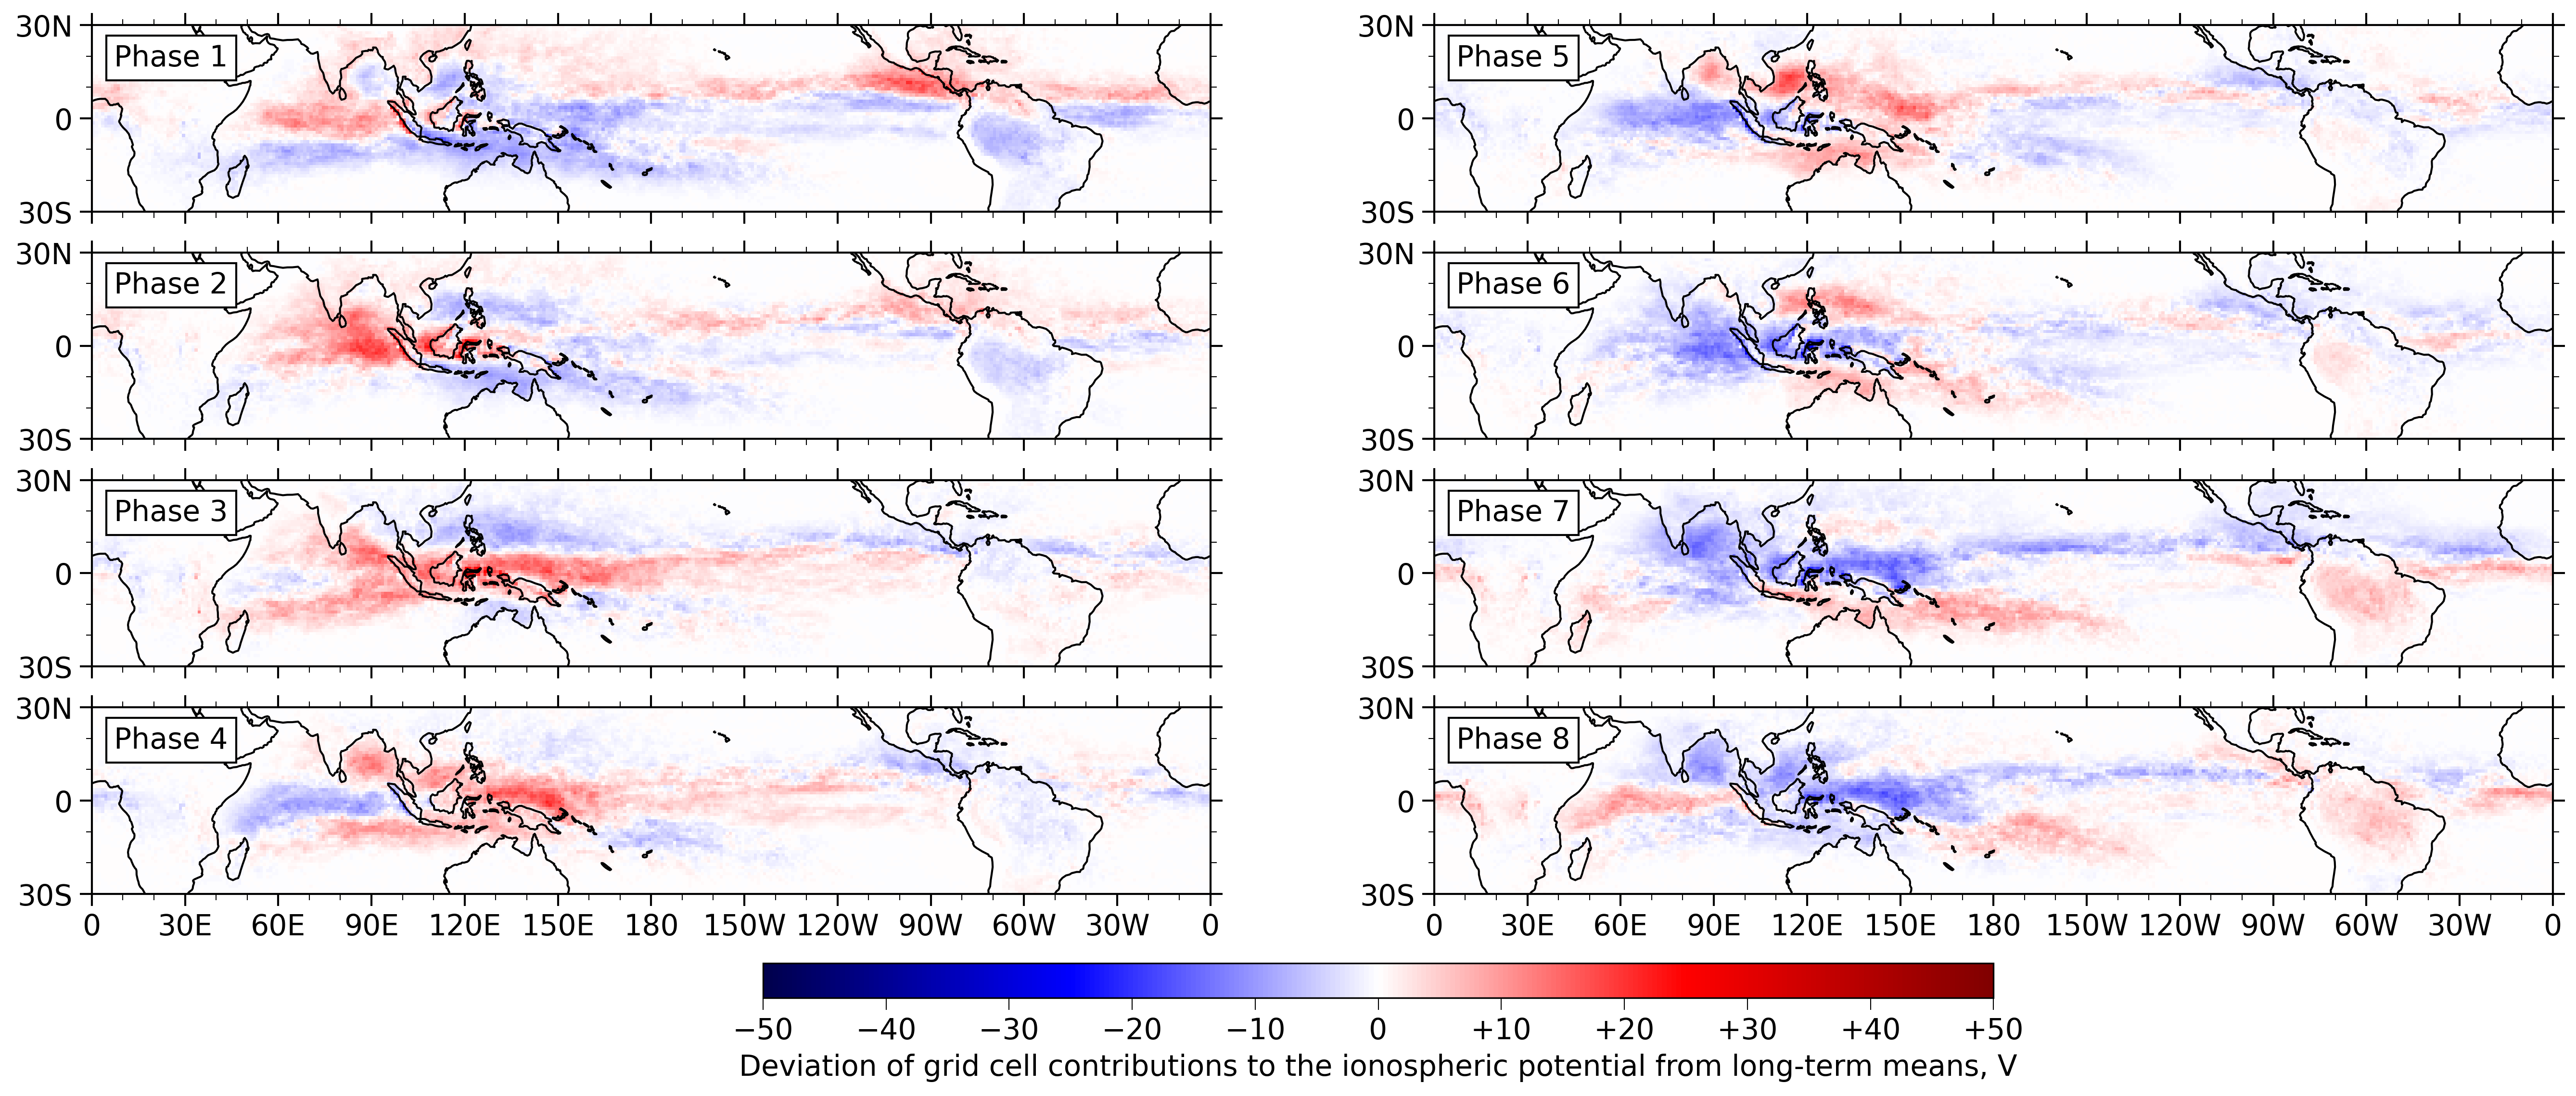
\includegraphics[width=\textwidth]{figures/map_of_contributions.png}
	\caption{Аномалии вкладов отдельных модельных столбцов в ИП в течение каждой из фаз КМД.}
	\label{fig:map_of_contributions}
\end{figure}

\begin{figure}[tb]
	\centering
	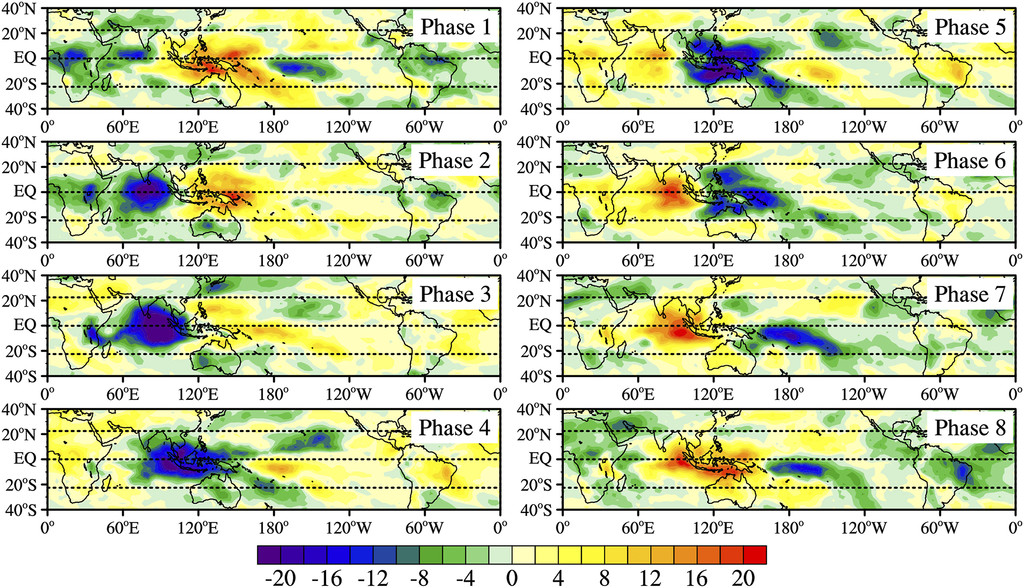
\includegraphics[width=\textwidth]{figures/map_of_olr_anomaly.jpg}
	\caption{Аномалии OLR ($\textnormal{Вт}/\textnormal{м}^2$) в течение каждой из фаз КМД за месяца зимы в северном полушарии (NDJF). Взяты лишь дни с амплитудой индекса RMM больше 1. Позаимствовано из \cite{Wang_et_al_2018}.}
	\label{fig:map_of_olr_anomaly}
\end{figure}

